\documentclass[tikz, 12pt]{standalone}

\usepackage{xcolor}
\definecolor{colora}{RGB}{214,76,71}
\definecolor{colorg}{RGB}{84,175,216}
\definecolor{colort}{RGB}{98,174,17}
\definecolor{colorc}{RGB}{253,205,103}
\definecolor{colorn}{RGB}{ 45,45,45}
\definecolor{colord}{RGB}{ 44,46,255}
\definecolor{colorb}{RGB}{ 14,41,89}
\definecolor{colori}{RGB}{255,44,45}

\usepackage{tikz}
\usetikzlibrary{arrows,shapes,backgrounds,shadows,calc,decorations.pathreplacing}

\tikzstyle{blockA} = [fill=colora, draw=black, ultra thick, rounded corners, drop shadow]
\tikzstyle{blockC} = [fill=colorc, draw=black, ultra thick, rounded corners, drop shadow]
\tikzstyle{blockG} = [fill=colorg, draw=black, ultra thick, rounded corners, drop shadow]
\tikzstyle{blockT} = [fill=colort, draw=black, ultra thick, rounded corners, drop shadow]
\tikzstyle{blockN} = [fill=colorn, draw=black, ultra thick, rounded corners, drop shadow]
\tikzstyle{blockd} = [fill=colord, draw=black, ultra thick, rounded corners, drop shadow]
\tikzstyle{blockb} = [fill=colorb, draw=black, ultra thick, rounded corners, drop shadow]
\tikzstyle{blocki} = [fill=colori, draw=black, ultra thick, rounded corners, drop shadow]


\tikzstyle{circleA} = [circle, inner color = colora!20, outer color=colora, draw=black, ultra thick, rounded corners, drop shadow]
\tikzstyle{circleC} = [circle, inner color = colorc!20, outer color=colorc, draw=black, ultra thick, rounded corners, drop shadow]
\tikzstyle{circleG} = [circle, inner color = colorg!20, outer color=colorg, draw=black, ultra thick, rounded corners, drop shadow]
\tikzstyle{circleT} = [circle, inner color = colort!20, outer color=colort, draw=black, ultra thick, rounded corners, drop shadow]
\tikzstyle{circleN} = [circle, inner color = colorn!20, outer color=colorn, draw=black, ultra thick, rounded corners, drop shadow]
\tikzstyle{circled} = [circle, inner color = colord!20, outer color=colord, draw=black, ultra thick, rounded corners, drop shadow]
\tikzstyle{circleb} = [circle, inner color = colorb!20, outer color=colorb, draw=black, ultra thick, rounded corners, drop shadow]
\tikzstyle{circlei} = [circle, inner color = colori!20, outer color=colori, draw=black, ultra thick, rounded corners, drop shadow]

\pgfmathdeclarerandomlist{randomColors}{
  {colora}
  {colorc}
  {colorg}
  {colort}
}

\begin{document}

\begin{tikzpicture}
  \begin{scope}[xshift=-6cm]
    \fill[white,fill opacity=0.6] (0,0) rectangle (5,5);
    \draw[black, dashed, ultra thick] (0,0) rectangle (5,5);
    \node[anchor=south]  at (2.5,0) {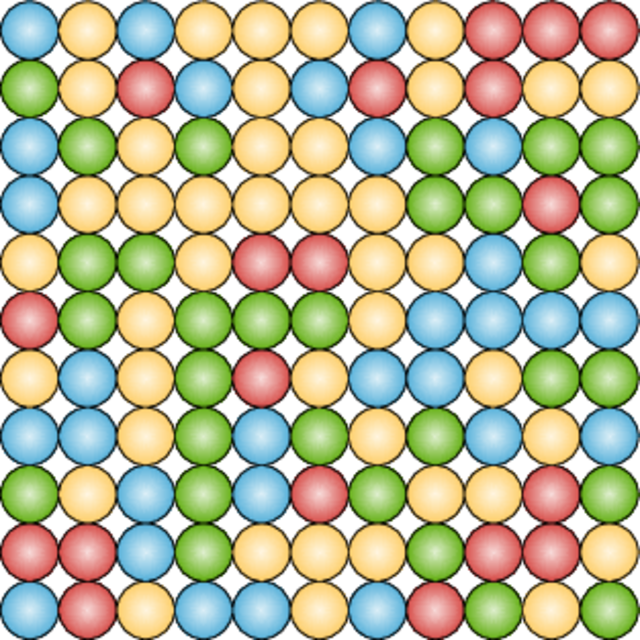
\includegraphics[width=5cm]{raw64.png}};
    \node[align=center, fill=colorn, drop shadow, ultra thick, text width=5cm, draw = black, text=white] (raw) at (2.5,5.5) {\bfseries{Raw data}};
  \end{scope} 

  
  \begin{scope}[xshift=0cm]
    \fill[white,fill opacity=0.9] (0,0) rectangle (5,5);
    \draw[black, dashed, ultra thick] (0,0) rectangle (5,5);
    \node[anchor=south]  at (2.5,0) {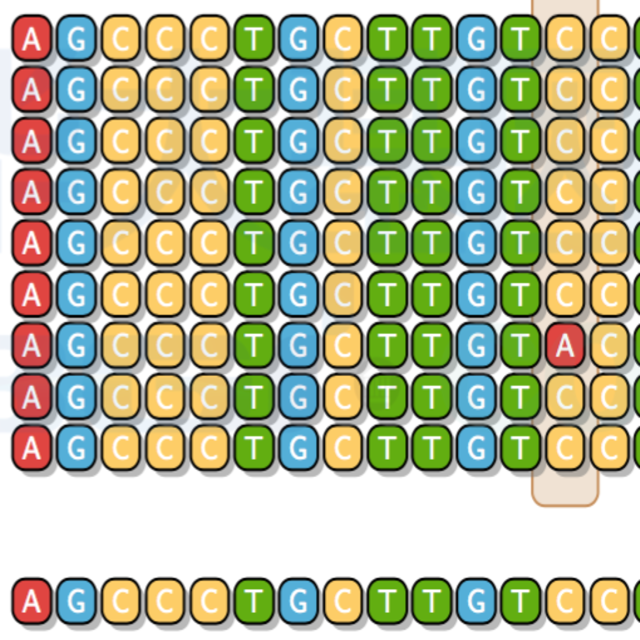
\includegraphics[width=5cm]{align64.png}};
    \node[align=center, fill=colorn, drop shadow, ultra thick, text width=5cm, draw = black, text=white] (alig) at (2.5,5.5) {\bfseries{Alignment}};
  \end{scope}

  \begin{scope}[xshift=6cm]
    \fill[white,fill opacity=.9] (0,0) rectangle (5,5);
    \draw[black, dashed, ultra thick] (0,0) rectangle (5,5);
    \node[anchor=south]  at (2.5,0) {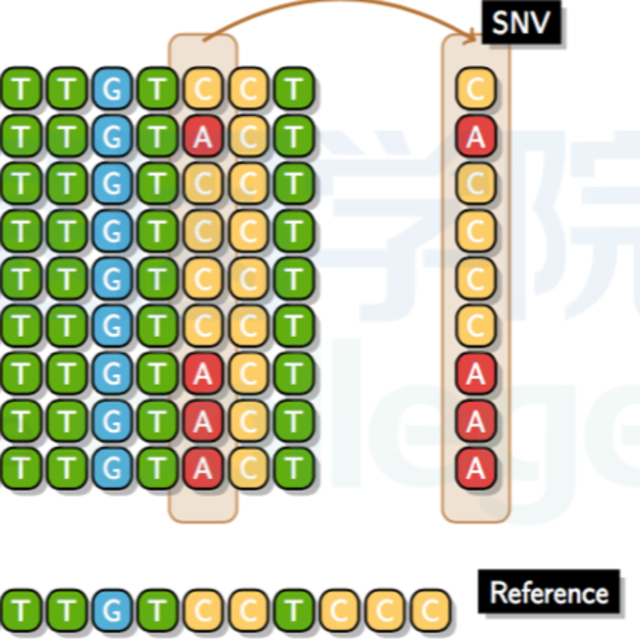
\includegraphics[width=5cm]{calling64.png}};
    \node[align=center, fill=colorn, drop shadow, ultra thick, text width=5cm, draw = black, text=white] (call) at (2.5,5.5) {\bfseries{Variants calling}};
  \end{scope}

  \begin{scope}[xshift=12cm]
    \fill[white,fill opacity=.9] (0,0) rectangle (5,5);
    \draw[black, dashed, ultra thick] (0,0) rectangle (5,5);
    \node[anchor=south]  at (2.5,0) {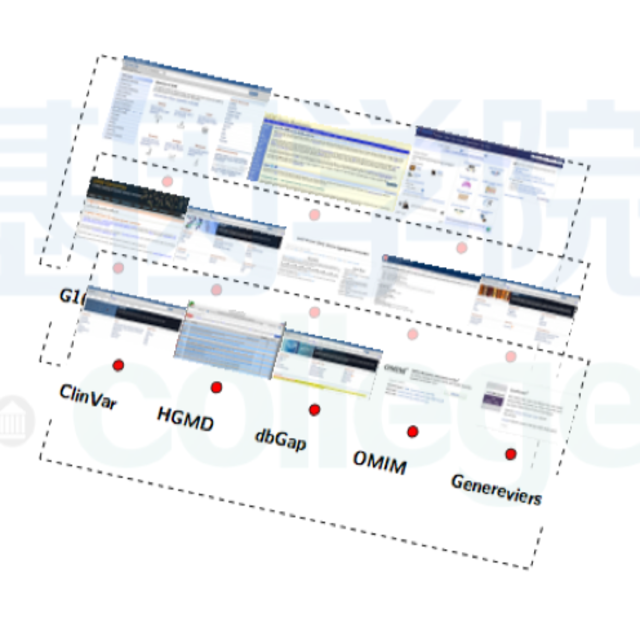
\includegraphics[width=5cm]{anno64.png}};
    \node[align = center, fill=colorn, drop shadow, ultra thick, draw = black, text=white, text width=5cm,] (anno) at (2.5,5.5) {\bfseries{Annotation}};

  \end{scope}

  \path[->, ultra thick, draw=colora] (raw) edge [in=90](alig);
  \path[->, ultra thick, draw=colora] (alig) edge [in=90] (call);
  \path[->, ultra thick, draw=colora] (call) edge [in=90](anno);
  
\end{tikzpicture}

\end{document}
